\documentclass{standalone}

\usepackage{hyperref}
\usepackage{tikz}

\usetikzlibrary{decorations.pathreplacing,
  arrows,
  calc,
  decorations.pathmorphing,
  decorations.pathreplacing,
  decorations.markings,
  positioning,
  shapes,
  3d
}

\tikzstyle{snakearrow} = [decorate, decoration={pre length=0.2cm,
  post length=0.2cm, snake, amplitude=.4mm,
  segment length=2mm},thick, ->]

\ifpdf
% Ensure reproducible output
\pdfinfoomitdate=1
\pdfsuppressptexinfo=-1
\pdftrailerid{}
\hypersetup{
  pdfcreator={},
  pdfproducer={}
}
\fi

\begin{document}
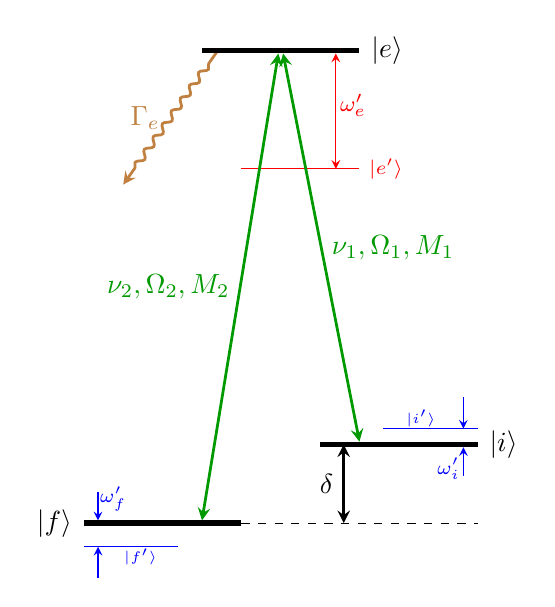
\begin{tikzpicture}
  \draw[line width=2] (2, 0) -- (0, 0) node[left] {$|f\rangle$};
  \draw[line width=2] (3, 1) -- (5, 1) node[right] {$|i\rangle$};

  \draw[->,>=stealth,snakearrow,brown,line width=1] (1.7, 6) -- node[left] {$\Gamma_e$} (0.5, 4.3);
  \draw[line width=2] (1.5, 6) -- (3.5, 6) node[right] {$|e\rangle$};

  \draw[dashed] (2, 0) -- (5, 0);
  \draw[<->,>=stealth,line width=1] (3.3, 0) -- node[left] {$\delta$} (3.3, 1);

  % \draw[blue] (3.8, 0.8) -- (5, 0.8);
  \draw[blue] (3.8, 1.2) -- node[above=-0.1,pos=0.4] {\tiny $|i'\rangle$} (5, 1.2);
  \draw[->,>=stealth,blue] (4.82, 1.6) -- (4.82, 1.2);
  \draw[->,>=stealth,blue] (4.82, 0.6) -- node[left=-0.08,pos=0.25] {\scriptsize $\omega'_i$} (4.82, 1.0cm - 1pt);

  \draw[blue] (0.0, -0.3) -- node[below=-0.1,pos=0.6] {\tiny $|f'\rangle$} (1.2, -0.3);
  % \draw[blue] (0.0, 0.3) -- (1.2, 0.3);
  \draw[->,>=stealth,blue] (0.18, -0.7) -- (0.18, -0.3);
  \draw[->,>=stealth,blue] (0.18, 0.4) -- node[right=-0.1,pos=0.25] {\scriptsize $\omega'_f$} (0.18, 0.0cm + 1pt);

  \draw[red] (2, 4.5) -- (3.5, 4.5) node[right] {\scriptsize $|e'\rangle$};
  \draw[<->,>=stealth,red] (3.2, 4.5) --
  node[right=-0.07, pos=0.55] {\footnotesize $\omega'_e$} (3.2, 6cm - 1pt);

  \draw[<->,>=stealth,green!60!black,line width=1] (3.5, 1cm + 1pt) -- node[right] {$\nu_1, \Omega_1, M_1$} (2.53, 6cm - 1pt);
  \draw[<->,>=stealth,green!60!black,line width=1] (1.5, 0cm + 1pt) -- node[left] {$\nu_2, \Omega_2, M_2$} (2.47, 6cm - 1pt);
\end{tikzpicture}
\end{document}
